\section{User Stories}

%4 --> Getting PDF output
\subsection{Getting PDF Output}
For this section, we performed a spike because we were not familiar specifically with the PDF format.

To do this spike, we built up a PDF file manually to simulate creating one programmatically. This was very difficult. PDF does not automatically create line breaks for text, so it is necessary for the user to determine when to break lines based on the size of the characters that appear on the line; in a non-monospace font, this means tracking the size of every character used in the font. PDF also uses a linked list data structure at the end of the document that stores a reference to every PDF object that appears in the document; to use this properly we would likely have to develop another data structure to store each PDF object we created as we wrote the document.

In conclusion, while writing PDF output is possible, it may not be technically feasible in the time frame that we have for this project, so we may need to focus only on generating HTML output.

%5 --> Outputting CSS
\hspace{-5cm}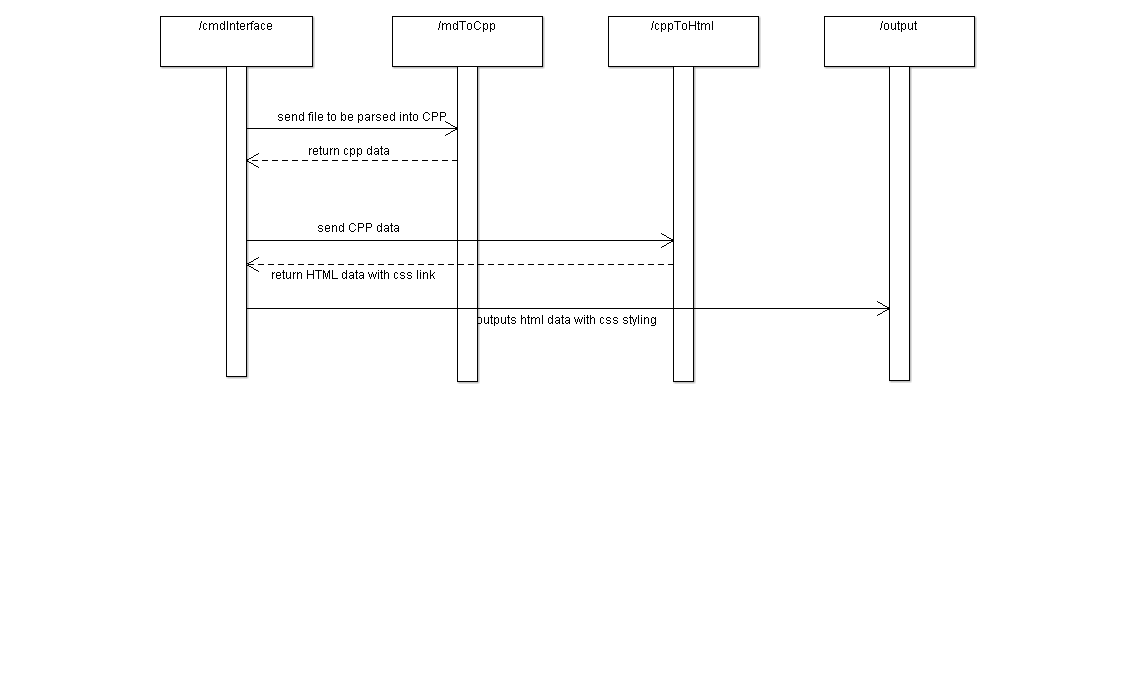
\includegraphics[width=700pt]{images/Output.png}

%6 --> Getting Help
\hspace{-2cm}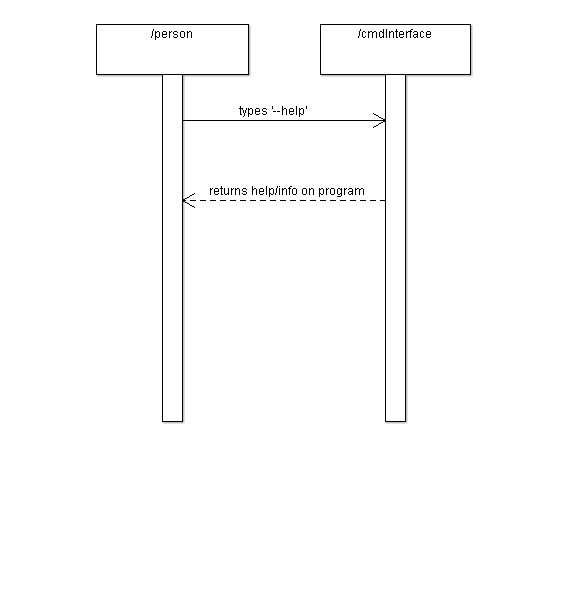
\includegraphics[width=450pt]{images/GettingHelp.png}

%7 --> Specifying the File
\hspace{-2cm}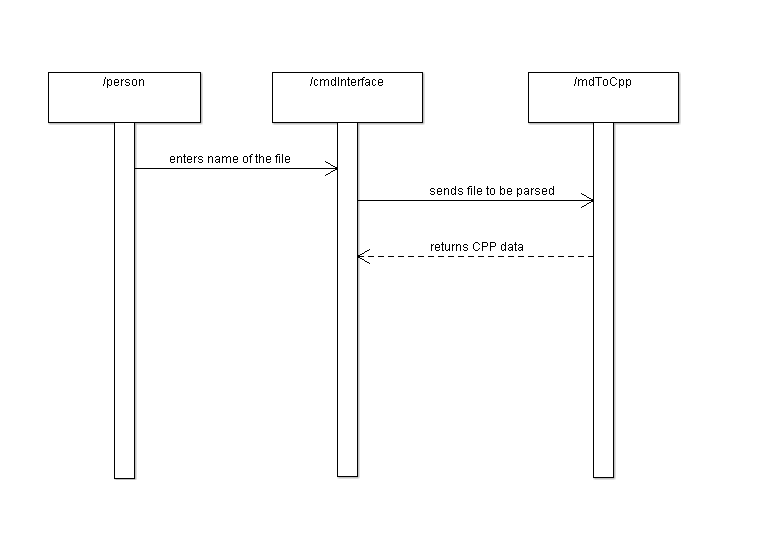
\includegraphics[width=500pt]{images/SpecifyingFile.png}

%8 --> Specifying the Output Type
\hspace{-3cm}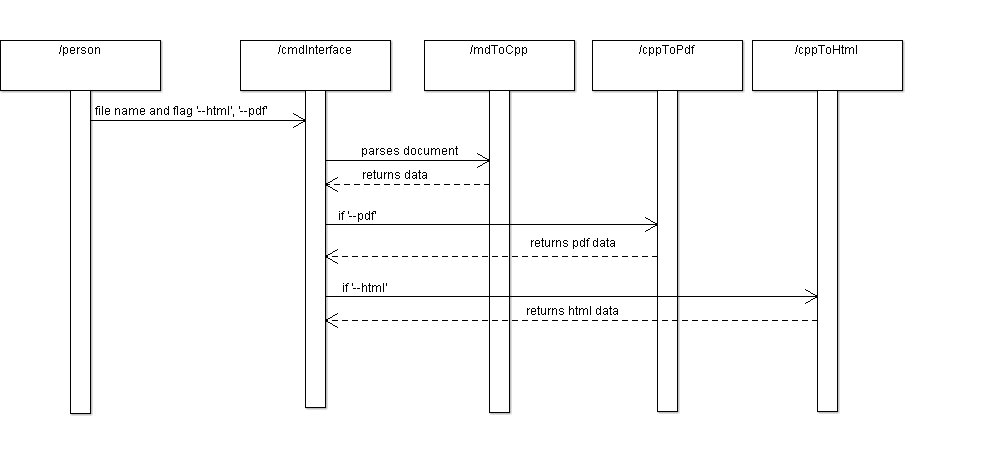
\includegraphics[width=550pt]{images/SpecifyingOutputFile.png}

%9 --> Specifying the Output Name 
\hspace{-3cm}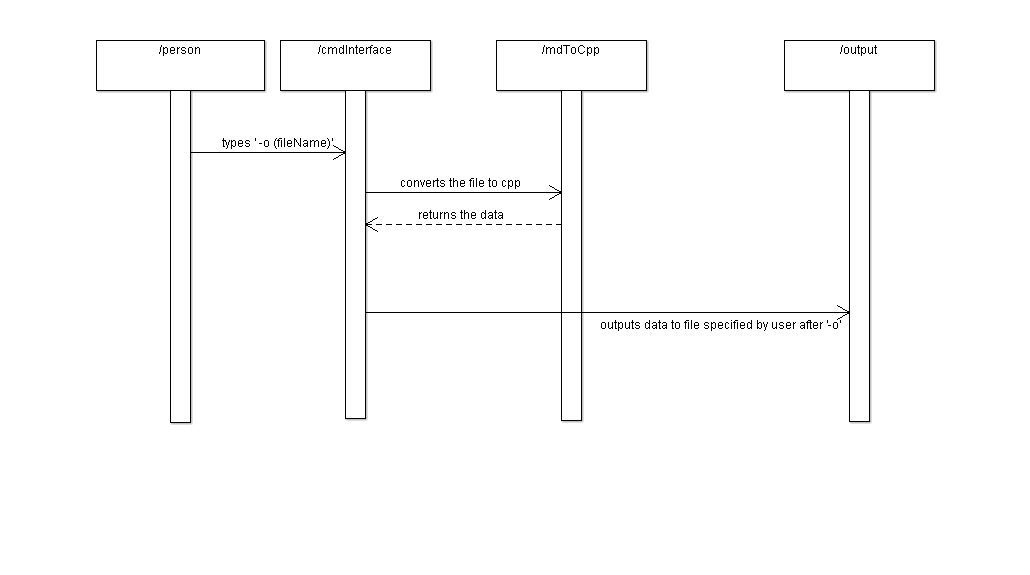
\includegraphics[width=500pt]{images/SpecifyingOutputName.png}
